
\de{ĐỀ THI HỌC KỲ II NĂM HỌC 2022-2023}{THPT Nguyễn Văn Tăng}
\begin{center}
	\textbf{PHẦN 1 - TRẮC NGHIỆM}
\end{center}
\Opensolutionfile{ans}[ans/ans]
%Câu 1...........................
\begin{ex}%[0T7Y1-1]%[Dự án đề kiểm tra HKII NH22-23- Võ Thị Thùy Trang]%[Nguyễn Văn Tăng]
	Tìm khẳng định đúng trong cac khẳng định sau.
	\choice
	{\True $f(x)=3 x^2+2 x-5$ là tam thức bậc hai}
	{ $f(x)=2 x-4$ là tam thức bậc hai}
	{$f(x)=3 x^3+2 x-1$ là tam thức bậc hai}
	{$f(x)=x^4-x^2+1$ là tam thức bậc hai}
	\loigiai{
		$f(x)=3 x^2+2 x-5$ là tam thức bậc hai.
	}
\end{ex}
%Câu 2...........................
\begin{ex}%[0T8Y1-2]%[Dự án đề kiểm tra HKII NH22-23- Võ Thị Thùy Trang]%[Nguyễn Văn Tăng]
	An muốn mua một cây bút mực và một cây bút chì. Các cây bút mực có $8$ màu khác nhau, các cây bút chì cũng có $8$ màu khác nhau. Như vậy An có bao nhiêu cách chọn?
	\choice
	{\True $64$}
	{$16$}
	{$32$}
	{$20$}
	\loigiai{
		\begin{itemize}
			\item Chọn một cây bút mực có $8$ cách.
			\item Chọn một cây bút chì có $8$ cách.
			\item Theo quy tắc nhân ta có $8\cdot 8=64$ cách chọn.
		\end{itemize}		
	}
\end{ex}
%Câu 3...........................
\begin{ex}%[0T8Y2-1]%[Dự án đề kiểm tra HKII NH22-23- Võ Thị Thùy Trang]%[Nguyễn Văn Tăng]
	Một ban chấp hành đoàn gồm $7$ người, cần chọn $3$ người vào ban thường vụ với các chức vụ là Bí thư, Phó bí thư, Ủy viên thì có bao nhiêu cách chọn?
	\choice
	{$120$}
	{\True $210$}
	{$35$}
	{$220$}
	\loigiai{
		Chọn $3$ người vào ban thường vụ với các chức vụ là Bí thư, Phó bí thư, Ủy viên thì có $\mathrm{A}_7^3=210$ cách chọn.
	}
\end{ex}
%Câu 4...........................
\begin{ex}%[0T8B2-1]%[Dự án đề kiểm tra HKII NH22-23- Võ Thị Thùy Trang]%[Nguyễn Văn Tăng]
	Một tổ có $6$ học sinh nữ và $9$ học sinh nam. Hỏi có bao nhiêu cách chọn $2$ học sinh nữ và $1$ học sinh nam đi lao động?
	\choice
	{$\mathrm{C}_9^2+\mathrm{C}_6^1$}
	{$\mathrm{C}_6^2+\mathrm{C}_9^1$}
	{\True $\mathrm{C}_6^2 \cdot \mathrm{C}_9^1$}
	{$\mathrm{C}_9^2 \cdot \mathrm{C}_6^1$}
	\loigiai{
		Chọn $2$ học sinh nữ và $1$ học sinh nam đi lao động có $\mathrm{C}_6^2 \cdot \mathrm{C}_9^1$ cách.
	}
\end{ex}
%Câu 5...........................
\begin{ex}%[0T8B2-1]%[Dự án đề kiểm tra HKII NH22-23- Võ Thị Thùy Trang]%[Nguyễn Văn Tăng]
	Một bàn có hai dãy ghế đối điện nhau, mỗi dãy $6$ ghế. Người ta xếp chỗ ngồi cho $6$ học sinh trường A và $6$ học sinh trường B vào bàn trên. Hỏi có bao nhiêu cách xếp để bất cứ hai học sinh nào ngồi đối diện nhau thì khác trường nhau?
	\choice
	{\True $1036800$}
	{$518400$}
	{$479001600$}
	{$33177600$}
	\loigiai{
		\begin{itemize}
			\item Số cách xếp $6$ học sinh trường A vào một dãy ghế là $6!$.
			\item Số cách xếp $6$ học sinh trường B vào một dãy ghế là $6!$.
			\item Số cách xếp để bất cứ hai học sinh ngồi đối diện nhau thì khác trường nhau là $$2\cdot 6!\cdot 6!=1036800.$$
		\end{itemize}
	}
\end{ex}
%Câu 6...........................
\begin{ex}%[0T9Y2-1]%[Dự án đề kiểm tra HKII NH22-23- Võ Thị Thùy Trang]%[Nguyễn Văn Tăng]
	Trong mặt phẳng $Oxy$, cho đường thẳng $(d)\colon 2x-3y+1=0$. Véc-tơ nào sau đây là một véc-tơ pháp tuyến của đường thẳng $(d)$?
	\choice
	{$\vec{n}=(3;2)$}
	{$\vec{n}=(-2;-3)$}
	{\True $\vec{n}=(2;-3)$}
	{$\vec{n}=(-3;2)$}
	\loigiai{
		Một véc-tơ pháp tuyến của đường thẳng $(d)$ là $\vec{n}=(2;-3)$.
	}
\end{ex}
%Câu 7...........................
\begin{ex}%[0T9Y2-2]%[Dự án đề kiểm tra HKII NH22-23- Võ Thị Thùy Trang]%[Nguyễn Văn Tăng]
	Trong mặt phẳng $Oxy$, đường thẳng đi qua điểm $M(1;2)$ và nhận $\vec{n}=(3;4)$ làm véc-tơ pháp tuyến có phương trình tổng quát là
	\choice
	{$3x-4y+5=0$}
	{\True $3x+4y-11=0$}
	{$x+2y-11=0$}
	{$4x+3y-10=0$}
	\loigiai{
		Đường thẳng đi qua điểm $M(1;2)$ và nhận $\vec{n}=(3;4)$ làm véc-tơ pháp tuyến có phương trình là $3(x-1)+4(y-2)=0$ hay $3x+4y-11=0$.
	}
\end{ex}
%Câu 8...........................
\begin{ex}%[0T9Y3-1]%[Dự án đề kiểm tra HKII NH22-23- Võ Thị Thùy Trang]%[Nguyễn Văn Tăng]
	Trong mặt phẳng $Oxy$, cho đường tròn $(C)\colon (x-2)^2+(y-3)^2=25$. Đường tròn $(C)$ có bán kính là
	\choice
	{$R=2$}
	{$R=3$}
	{$R=25$}
	{\True $R=5$}
	\loigiai{
		Đường tròn $(C)$ có bán kính là $R=5$.
	}
\end{ex}
%Câu 9...........................
\begin{ex}%[0T9B3-2]%[Dự án đề kiểm tra HKII NH22-23- Võ Thị Thùy Trang]%[Nguyễn Văn Tăng]
	Phương trình nào sau đây là phương trình của đường tròn có tâm $I(-4;5)$ và đi qua điểm $A(0;6)$?
	\choice
	{$x^2+(y-6)^2=17$}
	{$(x+4)^2+(y-5)^2=36$}
	{$(x-4)^2+(y+5)^2=36$}
	{\True $(x+4)^2+(y-5)^2=17$}
	\loigiai{ 
		Đường tròn có tâm $I(-4;5)$ và đi qua điểm $A(0;6)$ có bán kính là $$R=IA=\sqrt{(0+4)^2+(6-5)^2}=\sqrt{17}.$$
		Khi đó phương trình của đường tròn là $(x+4)^2+(y-5)^2=17$.
	}
\end{ex}
%Câu 10...........................
\begin{ex}%[Dự án đề kiểm tra HKII NH22-23- Võ Thị Thùy Trang]%[Nguyễn Văn Tăng]
	Parabol $(P)\colon y^2=20x$ có tham số tiêu là
	\choice
	{$p=20$}
	{$p=5$}
	{\True $p=10$}
	{$p=40$}
	\loigiai{
		Ta có $2p=20 \Rightarrow p=10$.\\
		Parabol $(P)\colon y^2=20x$ có tham số tiêu là $p=10$.
	}
\end{ex}


\Closesolutionfile{ans}
%\begin{center}
%	\textbf{ĐÁP ÁN}
%	\inputansbox{10}{ans/ans}	
%\end{center}


\begin{center}
	\textbf{PHẦN 2 - TỰ LUẬN}
\end{center}

\begin{bt}%[0T7B2-1]%[Đề thi HK2-THPT Nguyễn Văn Tăng, BCTuan]
	Giải bất phương trình $x^2-5x+6<0$.
	\loigiai{
Ta có $x^2-5x+6=0\Leftrightarrow \hoac{& x=2 \\ & x=3.}$\\
Bảng xét dấu của vế trái như sau
\begin{center}
	
\begin{tikzpicture}
		\tkzTabInit[lgt=3.5,espcl = 3,nocadre=false]
		{$x$ /0.8, $x^2-5x+6$ /0.8}
		{$-\infty$,$2$,$3$,$+\infty$}
		\tkzTabLine{ ,+,0,-,0, +, }
	\end{tikzpicture}
\end{center}
	Dựa vào bảng xét dấu, tập nghiệm của bất phương trình là $S=(2;3)$.
}
\end{bt}
\begin{bt}%[0T7B3-2]%[Đề thi HK2-THPT Nguyễn Văn Tăng, BCTuan]
	Giải phương trình sau: $\sqrt{x^2-6x+8}=\sqrt{3x+8}$.
	\loigiai{
Ta có 
\begin{eqnarray*}
	&&\sqrt{x^2-6x+8}=\sqrt{3x+8}\\
	&\Rightarrow &x^2-6x+8=3x+8\\
	&\Leftrightarrow &x^2-9x=0\\
	&\Leftrightarrow &\hoac{& x=0 \\ & x=9.}
\end{eqnarray*}	
Thay các nghiệm vừa tìm được vào phương trình ban đầu, ta thấy đều thỏa mãn.\\
Vậy tập nghiệm của phương trình là $S=\{0;9\}$.
}
\end{bt}
\begin{bt}%[0T7B2-1]%[Đề thi HK2-THPT Nguyễn Văn Tăng, BCTuan]
Bạn Hà cần làm một khung ảnh hình chữ nhật sao cho phần trong của khung là hình chữ nhật có kích thước $17\ \mathrm{cm} \times 25\ \mathrm{cm}$, độ rộng viền xung quanh là $x\  \mathrm{cm}$. Hỏi bạn Hà cần phải làm độ rộng viền khung ảnh tối đa bao nhiêu $\mathrm{cm}$ để diện tích của cả khung ảnh lớn nhất là $513\ \mathrm{cm}^2$?
\loigiai{
\immini
{
Chiều rộng của khung ảnh là $17+2x$ (cm).\\
Chiều dài của khung ảnh là $25+2x$ (cm).\\
Vì diện tích khung ảnh lớn nhất là $513$ cm$^2$ nên ta có
\begin{eqnarray*}
&&(17+2x)(25+2x)\le 513\\
&\Leftrightarrow& 4x^2+84x-88\le 0\\
&\Leftrightarrow& -22\le x\le 1.	
\end{eqnarray*}
Vậy độ rộng viền khung ảnh tối đa phải làm là $1$ cm.
}
{
	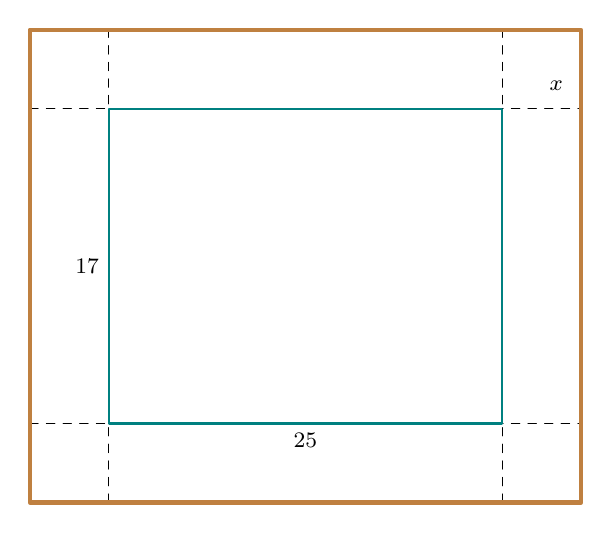
\begin{tikzpicture}[scale=1, font=\footnotesize, line join=round, line cap=round, >=stealth] 
	\path (1,1)--(6,1) node[midway,below]{$25$} (1,1)--(1,5) node[midway,left]{$17$};
	\draw[dashed] (1,0)--(1,6) (6,0)--(6,6) (0,1)--(7,1) (0,5)--(7,5) node[above left=3pt]{$x$};
		\draw[ultra thick, brown] (0,0) rectangle (7,6);\draw[thick,teal] (1,1) rectangle (6,5);
	\end{tikzpicture}
}
}
\end{bt}
\begin{bt}%[0T8B2-1]%[Đề thi HK2-THPT Nguyễn Văn Tăng, BCTuan]
	\begin{enumerate}
		\item Cho tập $A=\{0;1;2;3;4;5\}$. Từ tập $A$ có thể lập được bao nhiêu số tự nhiên có $4$ chữ số khác nhau và chia hết cho $5$?
		\item Một đoàn đại biểu có $5$ nhà Toán học, $6$ nhà Vật Lý. Chọn ra $5$ người, hỏi có bao nhiêu cách chọn sao cho có đúng $3$ nhà Toán học?
	\end{enumerate}
\loigiai{
\begin{enumerate}
	\item Giả sử số cần lập có dạng $\overline{abcd}$.\\
	{\bf TH1:} Với $d=0$, số cách chọn $\overline{abc}$ là $\mathrm{A}_5^3$ (cách).\\
	{\bf TH2:} Với $d=5$, số cách chọn $a$ là $4$ cách, số cách chọn $\overline{bc}$ là $\mathrm{A}_4^2$ (cách).\\
	Vậy số các số tự nhiên thỏa mãn là $\mathrm{A}_5^3+4\cdot \mathrm{A}_4^2=108$ (số).
	\item Số cách chọn ra $3$ nhà Toán học là $\mathrm{C}_5^3$ (cách).\\
	Số cách chọn ra $2$ nhà Vật Lý là  $\mathrm{C}_6^2$ (cách).\\
	Theo quy tắc nhân, số cách chọn thỏa mãn là $\mathrm{C}_6^2\cdot \mathrm{C}_5^3=150$ (cách).
\end{enumerate}
}
\end{bt}




\begin{bt}%[0T8K3-2]%[Dự án đề kiểm tra HKII NH22-23- Phạm Duy Phương]%[THPT Nguyễn Văn Tăng-Sở Hồ Chí Minh]
	Tìm số hạng chứa $x^7$ trong khai triển $\left(\dfrac{2}{x}-x^3\right)^5$, $x \neq 0$.
\loigiai{
	\allowdisplaybreaks \begin{eqnarray*}
		\left(\dfrac{2}{x}-x^3\right)^5&=&\mathrm{C}_5^0\cdot \left(\dfrac{2}{x}\right)^5\cdot \left(-x^3\right)^0+\mathrm{C}_5^1\cdot \left(\dfrac{2}{x}\right)^4\cdot \left(-x^3\right)^1+\mathrm{C}_5^2\cdot \left(\dfrac{2}{x}\right)^3\cdot \left(-x^3\right)^2\\
		&&+\mathrm{C}_5^3\cdot \left(\dfrac{2}{x}\right)^2\cdot \left(-x^3\right)^3+\mathrm{C}_5^4\cdot \left(\dfrac{2}{x}\right)^1\cdot \left(-x^3\right)^4+\mathrm{C}_5^5\cdot \left(\dfrac{2}{x}\right)^0\cdot \left(-x^3\right)^5\\
		&=&\dfrac{32}{x^5}-5\cdot \dfrac{16}{x^4}\cdot x^3+10\cdot\dfrac{8}{x^3}\cdot x^6-10\cdot \dfrac{4}{x^2}\cdot x^9+5\cdot \dfrac{2}{x}\cdot x^{12}-x^{15}\\
		&=&\dfrac{32}{x^5}-\dfrac{80}{x}+80x^3-40x^7+10x^{11}-x^{15}.
	\end{eqnarray*}
	Vậy số hạng chứa $x^7$ là $-40x^7$.
}
\end{bt}
\begin{bt}%[0T9K2-2]%[0T9K3-2]%[Dự án đề kiểm tra HKII NH22-23- Phạm Duy Phương]%[THPT Nguyễn Văn Tăng-Sở Hồ Chí Minh]
	Trong mặt phẳng tọa độ $Oxy$, cho tam giác $ABC$ biết $A(1;-3)$, $B(4;0)$, $C(2;-6)$.
	\begin{enumerate}
		\item Viết phương trình đường cao $AH$ của tam giác $ABC$.
		\item Viết phương trình đường tròn có đường kính $BC$.
	\end{enumerate}
	\loigiai{
\begin{enumerate}
	\item Ta có $\vec{BC}=\left(2-4;-6-0\right)=\left(-2;-6\right)$.\\
	Đường cao $AH$ qua $A(1;-3)$ và vuông góc với $BC$ nên nhận $\vec{BC}$ làm véc-tơ pháp tuyến. Phương trình đường cao $AH$ có dạng
	\allowdisplaybreaks
	\begin{eqnarray*}
		& &-2\left(x-1\right)-6\left(y-(-3)\right)=0\\
		&\Leftrightarrow &  -2x+2-6y-18=0\\
		&\Leftrightarrow & -2x-6y-16=0 \Leftrightarrow x+3y+8=0.
	\end{eqnarray*}
	\item Đường tròn đường kính $BC$ có tâm $I$ là trung điểm của $BC$ và bán kính là $R=\dfrac{BC}{2}$.
	\begin{itemize}
		\item Trung điểm của $BC$ là $I(3;-3)$.
		\item $R=\dfrac{BC}{2}=\dfrac{\sqrt{(2-4)^2+(-6-0)^2}}{2}=\sqrt{10}$.
	\end{itemize}
Vậy phương trình đường tròn có đường kính $BC$ có dạng
\allowdisplaybreaks
\begin{eqnarray*}
	& &\left(x-3\right)^2+\left(y-(-3)\right)^2=\left(\sqrt{10}\right)^2 \\
	&\Leftrightarrow &\left(x-3\right)^2+\left(y+3\right)^2=10.
\end{eqnarray*}
\end{enumerate}	
}
\end{bt}
\begin{bt}%[0T9G3-3]%[0T9B4-2]%[Dự án đề kiểm tra HKII NH22-23- Phạm Duy Phương]%[THPT Nguyễn Văn Tăng-Sở Hồ Chí Minh]
	\begin{enumerate}
		\item Viết phương trình tiếp tuyến của đường tròn $(C)\colon (x-5)^2+(y-1)^2=16$, biết tiếp tuyến song song với đường thẳng $\Delta\colon 3x+4y+1=0$.
		\item Viết phương trình của đường elip $(E)$, biết độ dài trục lớn bằng $10$ và tiêu cự bằng $4$.
	\end{enumerate}
	\loigiai{
\begin{enumerate}
	\item Đường tròn $(C)\colon (x-5)^2+(y-1)^2=16$ có tâm $I\left(5;1\right)$ và bán kính là $R=\sqrt{16}=4$.\\
	Gọi tiếp tuyến cần tìm là $d$. Vì $d\parallel \Delta$ nên $d$ có phương trình dạng
	$$3x+4y+c=0\quad (c\neq 1).$$
	Lại có
	\allowdisplaybreaks\begin{eqnarray*}
		\mathrm{d}\left(I,d\right)=R&\Leftrightarrow&\dfrac{\left|3\cdot 5+4\cdot 1+c\right|}{\sqrt{3^2+4^2}}=4 \\
		&\Leftrightarrow & \left|19+c\right|=20 \Leftrightarrow \hoac{&c=1&\text{(không thoả mãn)}\\&c=-39&\text{(thoả mãn).}}
	\end{eqnarray*}
Vậy tiếp tuyến cần tìm là $d\colon 3x+4y-39=0$.
\item Gọi elip $(E)$ có phương trình dạng $\dfrac{x^2}{a^2}+\dfrac{y^2}{b^2}=1$.
\begin{itemize}
	\item Độ dài trục lớn bằng $10$ $\Rightarrow 2a=10 \Leftrightarrow a=5$.
	\item Tiêu cự bằng $4$ $\Rightarrow 2c=4 \Leftrightarrow c=2$.
\end{itemize}
$\Rightarrow b^2=a^2-c^2=5^2-2^2=21$.\\
Vậy elip $(E)$ có phương trình dạng $\dfrac{x^2}{25}+\dfrac{y^2}{21}=1$.
\end{enumerate}	
}
\end{bt}

